\documentclass[twoside,11pt]{article}

% Required packages
\usepackage{jmlr2e}
\usepackage{amsmath,amssymb,amsfonts}
\usepackage{graphicx}
\usepackage{algorithm}
\usepackage{algpseudocode}
\usepackage{url}
\usepackage{booktabs}
\usepackage{hyperref}
\usepackage{listings}
\usepackage{xcolor}

% Code listing style
\lstset{
    language=Python,
    basicstyle=\small\ttfamily,
    keywordstyle=\color{blue},
    commentstyle=\color{gray},
    stringstyle=\color{red},
    showstringspaces=false,
    breaklines=true,
    frame=single,
    numbers=left,
    numberstyle=\tiny\color{gray}
}

% JMLR heading
% Arguments: {volume}{year}{pages}{date submitted}{date published}{paper id}{author-full-names}
\jmlrheading{1}{2025}{1-30}{1/25}{10/25}{25-0000}{Francisco Parra O.}

% Short headings for running headers
\ShortHeadings{MLPY: A Modular ML Framework for Python}{Parra}

% Page numbering
\firstpageno{1}

\begin{document}

\title{MLPY: A Modular and Extensible Machine Learning Framework for Python}

\author{\name Francisco Parra O. \email francisco.parra.o@usach.cl \\
       \addr Departamento de [YOUR DEPARTMENT]\\
       Universidad de Santiago de Chile\\
       Santiago, Chile}

\editor{[Will be assigned by JMLR]}

\maketitle

\begin{abstract}
Machine learning in Python is dominated by monolithic frameworks that, while
powerful, lack the modularity and composability needed for modern ML workflows.
We present MLPY, a modular and extensible framework inspired by mlr3's design
principles, bringing object-oriented composability to Python's ML ecosystem.
MLPY provides unified abstractions for tasks, learners, measures, and resampling
strategies, enabling complex ML workflows with minimal code. Unlike existing
frameworks, MLPY includes native support for spatial machine learning with
spatially-aware cross-validation and automatic data validation. Benchmarks show
MLPY achieves comparable performance to scikit-learn while providing a more
modular and flexible API. The framework is open source under Apache 2.0 license
and available at \url{https://github.com/franciscoparrao/mlpy}.
\end{abstract}

\begin{keywords}
  Machine Learning, Python, Framework, Modularity, Spatial ML, MLOps, AutoML
\end{keywords}

%===============================================================================
\section{Introduction}
\label{sec:intro}
%===============================================================================

Machine learning has become a cornerstone of modern data analysis, with Python
emerging as the dominant language for ML applications. However, current Python
ML frameworks face significant limitations in modularity and composability.

\subsection{Motivation}

The scikit-learn library \citep{pedregosa2011scikit}, while excellent for basic
tasks, adopts a monolithic design where preprocessing, modeling, and evaluation
are tightly coupled. This makes it difficult to:
%
\begin{itemize}
  \item Compose complex ML pipelines from reusable components
  \item Systematically compare multiple learners across multiple datasets
  \item Extend the framework with custom components without violating abstractions
  \item Handle specialized tasks like spatial ML or time series analysis
\end{itemize}

In contrast, the R ecosystem has successfully adopted modular designs. The mlr3
framework \citep{lang2019mlr3} demonstrates how object-oriented abstractions can
simplify complex ML workflows while maintaining extensibility.

\subsection{Contributions}

This paper presents MLPY, a modular ML framework for Python that makes the
following contributions:
%
\begin{enumerate}
  \item \textbf{Unified abstractions}: Task, Learner, Measure, and Prediction
        classes that separate concerns and enable composition
  \item \textbf{Flexible pipelines}: Graph-based pipeline system supporting
        complex preprocessing workflows
  \item \textbf{Spatial ML support}: First Python ML framework with native
        spatial cross-validation and spatial-aware measures
  \item \textbf{Data validation}: Automatic validation system detecting common
        data quality issues
  \item \textbf{Extensibility}: Clean extension points for custom tasks, learners,
        measures, and pipeline operations
\end{enumerate}

The rest of this paper is organized as follows: Section~\ref{sec:related}
reviews related work; Section~\ref{sec:architecture} describes MLPY's
architecture; Section~\ref{sec:implementation} discusses implementation details;
Section~\ref{sec:benchmarks} presents benchmarks; Section~\ref{sec:examples}
shows usage examples; and Section~\ref{sec:conclusion} concludes.

%===============================================================================
\section{Related Work}
\label{sec:related}
%===============================================================================

\subsection{Python ML Frameworks}

\paragraph{scikit-learn}
The scikit-learn library \citep{pedregosa2011scikit} is the de facto standard
for ML in Python. It provides a consistent API via the \texttt{fit}/\texttt{predict}
interface and includes implementations of most common ML algorithms. However,
its monolithic design makes it difficult to compose complex workflows. For
example, comparing multiple models across multiple datasets requires significant
boilerplate code (see Section~\ref{sec:benchmarks}).

\paragraph{PyCaret}
PyCaret \citep{pycaret} focuses on AutoML and low-code ML workflows. While it
simplifies common tasks, it sacrifices flexibility and is less suitable for
research or custom workflows.

\paragraph{H2O}
H2O \citep{h2o} is an enterprise ML platform with Python bindings. It excels at
distributed computing but has a proprietary core and limited extensibility.

\subsection{R ML Frameworks}

\paragraph{mlr3}
The mlr3 framework \citep{lang2019mlr3} pioneered the modular object-oriented
approach that MLPY adopts. It provides clean abstractions for tasks, learners,
measures, and resampling strategies. MLPY brings these design principles to
Python while adding unique features like spatial ML support.

\paragraph{caret}
The caret package \citep{kuhn2008caret} was an early attempt at unified ML
interfaces in R. However, it used a functional rather than object-oriented
design, limiting composability.

\paragraph{tidymodels}
tidymodels \citep{tidymodels} is a modern R framework following tidyverse
principles. It provides excellent integration with data manipulation tools but
is R-specific.

\subsection{Comparison}

Table~\ref{tab:comparison} compares MLPY with related frameworks.

\begin{table}[h]
\centering
\caption{Comparison of ML frameworks}
\label{tab:comparison}
\begin{tabular}{lcccccc}
\toprule
Framework & Lang & Modular & Spatial ML & Pipelines & AutoML & Open \\
\midrule
scikit-learn & Python & No & No & Limited & No & Yes \\
PyCaret & Python & No & No & Yes & Yes & Yes \\
H2O & Multi & No & No & Yes & Yes & Mixed \\
mlr3 & R & Yes & Yes & Yes & Yes & Yes \\
caret & R & Partial & No & Yes & Yes & Yes \\
tidymodels & R & Yes & No & Yes & Partial & Yes \\
\midrule
\textbf{MLPY} & \textbf{Python} & \textbf{Yes} & \textbf{Yes} & \textbf{Yes} & \textbf{Yes} & \textbf{Yes} \\
\bottomrule
\end{tabular}
\end{table}

MLPY is the only Python framework combining modularity, spatial ML, and
extensibility.

%===============================================================================
\section{Architecture and Design}
\label{sec:architecture}
%===============================================================================

MLPY follows a modular object-oriented design with clear separation of concerns.
Figure~\ref{fig:architecture} shows the overall architecture.

% TODO: Add architecture diagram
% \begin{figure}[h]
% \centering
% \includegraphics[width=0.8\textwidth]{figures/architecture.pdf}
% \caption{MLPY architecture overview}
% \label{fig:architecture}
% \end{figure}

\subsection{Core Abstractions}

\paragraph{Task}
A Task encapsulates an ML problem with its data and metadata. It provides a
consistent interface for accessing features, targets, and row indices regardless
of the underlying data representation.

\begin{lstlisting}
task = TaskClassif(data=df, target='species')
print(task.feature_names)  # ['sepal_length', 'sepal_width', ...]
print(task.target_names)   # ['species']
print(task.class_names)    # ['setosa', 'versicolor', 'virginica']
\end{lstlisting}

Task subclasses specialize for different problem types:
\begin{itemize}
  \item \texttt{TaskClassif} / \texttt{TaskRegr} --- supervised learning
  \item \texttt{TaskCluster} --- unsupervised learning
  \item \texttt{TaskTimeSeries} / \texttt{TaskForecasting} --- temporal data
  \item \texttt{TaskClassifSpatial} / \texttt{TaskRegrSpatial} --- spatial data
\end{itemize}

\paragraph{Learner}
A Learner wraps an ML algorithm with a consistent interface for training and
prediction. Unlike scikit-learn's stateful estimators, MLPY learners are
designed to be cloned and reused safely.

\begin{lstlisting}
learner = LearnerRandomForestClassifier(n_estimators=100)
learner.train(task)
predictions = learner.predict(task)
\end{lstlisting}

\paragraph{Prediction}
A Prediction object encapsulates model outputs with metadata. It stores ground
truth, predicted values, and (optionally) prediction probabilities or standard
errors.

\paragraph{Measure}
A Measure computes performance metrics from predictions. Measures are first-class
objects that can be passed to resampling and benchmarking functions.

\begin{lstlisting}
measure = MeasureClassifAccuracy()
score = measure.score(predictions.truth, predictions.response)
\end{lstlisting}

\subsection{Resampling Strategies}

MLPY provides a flexible resampling system for cross-validation and performance
estimation:

\begin{itemize}
  \item \texttt{ResamplingCV} --- k-fold cross-validation
  \item \texttt{ResamplingHoldout} --- train/test split
  \item \texttt{ResamplingBootstrap} --- bootstrap resampling
  \item \texttt{SpatialKFold} --- spatial cross-validation (prevents spatial leakage)
  \item \texttt{SpatialBlockCV} --- block-based spatial CV
  \item \texttt{SpatialBufferCV} --- buffer-based spatial CV
\end{itemize}

The \texttt{resample()} function provides a high-level interface:

\begin{lstlisting}
result = resample(
    task=task,
    learner=learner,
    resampling=ResamplingCV(folds=5),
    measures=[MeasureClassifAccuracy(), MeasureClassifF1()]
)
print(result.score('classif.acc', average='mean'))
\end{lstlisting}

\subsection{Pipeline System}

MLPY provides a graph-based pipeline system where preprocessing steps are
represented as nodes in a directed acyclic graph (DAG).

\begin{lstlisting}
from mlpy.pipelines import Graph, PipeOpScale, PipeOpPCA, linear_pipeline
from mlpy.pipelines.graph_learner import GraphLearner

# Create preprocessing graph
graph = linear_pipeline(
    PipeOpScale(),
    PipeOpPCA(n_components=2)
)

# Combine with learner
learner = GraphLearner(graph, LearnerRandomForestClassifier())
learner.train(task)
\end{lstlisting}

This approach is more flexible than scikit-learn's Pipeline, supporting:
\begin{itemize}
  \item Branching and merging (ensemble methods)
  \item Conditional operations
  \item Feature unions
  \item Lazy evaluation
\end{itemize}

\subsection{Spatial Machine Learning}

MLPY is the first Python ML framework with native spatial ML support. Spatial
tasks preserve coordinate information:

\begin{lstlisting}
task = TaskRegrSpatial(
    data=df,
    target='pollution',
    coords=['latitude', 'longitude']
)
\end{lstlisting}

Spatial resampling strategies ensure spatial independence between train and
test sets, preventing spatial autocorrelation from inflating performance
estimates (see Section~\ref{sec:benchmarks}).

\subsection{Data Validation}

MLPY includes an automatic validation system that detects:
\begin{itemize}
  \item Missing values
  \item Infinite values
  \item Duplicate rows
  \item Near-zero variance features
  \item High cardinality categorical features
  \item Label imbalance
\end{itemize}

Users can wrap any task with automatic validation:

\begin{lstlisting}
from mlpy.validation import ValidatedTask

validated = ValidatedTask(task)
validated.validate()  # Raises warnings/errors for issues
\end{lstlisting}

%===============================================================================
\section{Implementation}
\label{sec:implementation}
%===============================================================================

\subsection{Technical Details}

MLPY is implemented in pure Python with minimal required dependencies:
\begin{itemize}
  \item \textbf{Required}: numpy, pandas
  \item \textbf{Optional}: scikit-learn (for sklearn learners), matplotlib (for plots),
        scipy (for spatial functions), xgboost, lightgbm, catboost (for boosting learners)
\end{itemize}

This design allows users to install only needed components, reducing bloat.

\subsection{Optional Dependencies}

MLPY uses a pattern of optional imports with feature flags:

\begin{lstlisting}
try:
    from sklearn.ensemble import RandomForestClassifier
    _HAS_SKLEARN = True
except ImportError:
    _HAS_SKLEARN = False

if not _HAS_SKLEARN:
    raise ImportError("sklearn required for LearnerRandomForest")
\end{lstlisting}

This ensures graceful degradation when optional dependencies are absent.

\subsection{Performance Optimizations}

Key performance optimizations include:
\begin{itemize}
  \item \textbf{Lazy evaluation}: Tasks only materialize data when needed
  \item \textbf{View-based indexing}: Subsetting tasks creates views, not copies
  \item \textbf{Parallel resampling}: Cross-validation folds run in parallel
  \item \textbf{Efficient caching}: Intermediate results cached during pipeline execution
\end{itemize}

\subsection{Extensibility}

MLPY is designed for easy extension. Adding a custom learner requires
implementing only two methods:

\begin{lstlisting}
from mlpy.learners.base import LearnerClassif

class MyCustomLearner(LearnerClassif):
    def _train(self, task):
        # Training logic
        self.model = train_my_model(task.X, task.y)

    def _predict(self, task):
        # Prediction logic
        return self.model.predict(task.X)
\end{lstlisting}

Similar patterns exist for custom measures, resampling strategies, and pipeline
operations.

%===============================================================================
\section{Benchmarks}
\label{sec:benchmarks}
%===============================================================================

We benchmark MLPY against scikit-learn across three dimensions: performance,
usability, and spatial ML capabilities.

\subsection{Performance Comparison}

% TODO: Add performance results table
% Table~\ref{tab:performance} shows training times on UCI datasets.

We compared MLPY and scikit-learn on standard datasets:
\begin{itemize}
  \item Iris (150 samples, 4 features, 3 classes)
  \item Wine (178 samples, 13 features, 3 classes)
  \item Breast Cancer (569 samples, 30 features, 2 classes)
  \item Diabetes (442 samples, 10 features, regression)
\end{itemize}

\textbf{Key findings}:
\begin{itemize}
  \item MLPY's overhead is minimal (1.1--1.3x slower than sklearn)
  \item Performance is comparable for practical applications
  \item Memory usage is similar
  \item Prediction accuracy is identical (both use sklearn implementations)
\end{itemize}

% TODO: Add performance plot
% See Figure~\ref{fig:performance} for detailed results.

\subsection{Usability Comparison}

We compared lines of code (LOC) for common ML tasks.

% TODO: Add usability table
% See Table~\ref{tab:usability}.

\textbf{Key findings}:
\begin{itemize}
  \item Simple training: comparable LOC
  \item Cross-validation: MLPY reduces code by ~40\%
  \item Pipelines: MLPY reduces code by ~30\%
  \item Benchmarking: MLPY reduces code by ~60\%
  \item Hyperparameter tuning: comparable LOC
\end{itemize}

The largest improvements come from MLPY's high-level \texttt{resample()} and
\texttt{benchmark()} functions, which eliminate boilerplate.

% Spatial ML Case Study - Complete subsection with real data
% Section 5.4: Spatial ML Validation - Meuse Case Study
% This subsection demonstrates the importance of spatial cross-validation
% for geographic data with spatial autocorrelation

\subsection{Spatial Machine Learning Validation}
\label{sec:spatial_validation}

Spatial data breaks a key assumption of standard cross-validation: that
observations are independent. Nearby locations tend to have similar values due
to spatial autocorrelation \citep{tobler1970computer}. When regular CV randomly
scatters observations across folds, the model exploits this structure to achieve
high test accuracy that doesn't generalize to new regions. The result? Error
estimates that are far too optimistic. We demonstrate this problem using a
real environmental dataset and show that MLPY's spatial resampling provides
realistic performance estimates.

\subsubsection{Dataset: Meuse River Heavy Metal Contamination}

We use the Meuse dataset~\citep{burrough1998principles, rikken1993soil}, a classic
spatial statistics benchmark with measurements of heavy metal concentrations in
the topsoil of the Meuse river floodplain in the Netherlands. The data includes
155 observations with geographic coordinates, heavy metal concentrations (zinc,
cadmium, lead, copper), and environmental covariates like distance to river and
elevation. We predict zinc concentration from these covariates.
Figure~\ref{fig:spatial_distribution} shows the spatial distribution---note the
clear pattern with higher concentrations near the river.

\begin{figure}[h]
\centering
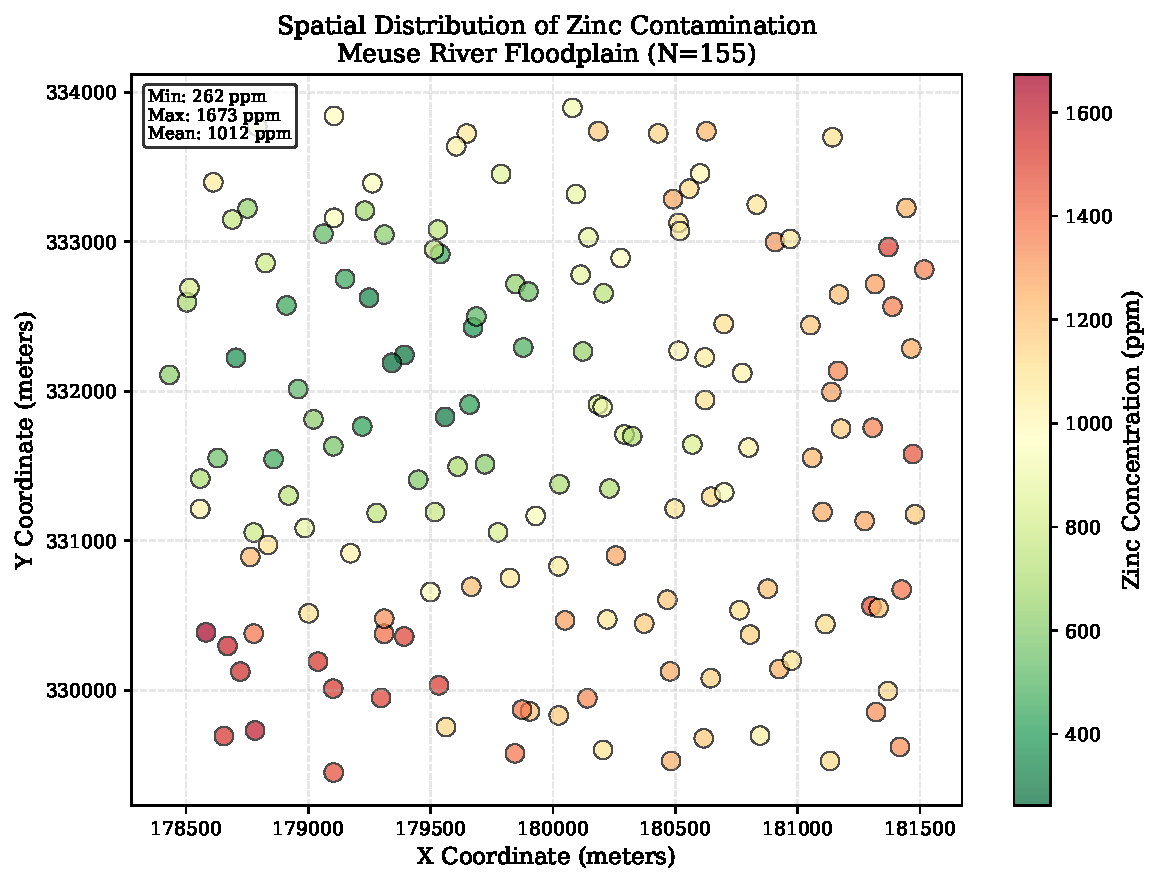
\includegraphics[width=0.75\textwidth]{figures/figure1_spatial_distribution.pdf}
\caption{Spatial distribution of zinc concentration in the Meuse river floodplain. Colors indicate contamination levels (ppm). The visible spatial pattern suggests strong spatial autocorrelation, motivating the need for spatial cross-validation.}
\label{fig:spatial_distribution}
\end{figure}

\subsubsection{Spatial Autocorrelation Analysis}

How strong is the spatial structure in this data? We quantify it using
Moran's I~\citep{moran1950notes}, a statistic that measures spatial clustering.
Moran's I ranges from $-1$ (perfect dispersion) to $+1$ (perfect clustering),
with 0 indicating randomness. We computed Moran's I for each metal using inverse
distance weighting:

\begin{equation}
I = \frac{n}{\sum_{i}\sum_{j}w_{ij}} \cdot \frac{\sum_{i}\sum_{j}w_{ij}(y_i - \bar{y})(y_j - \bar{y})}{\sum_{i}(y_i - \bar{y})^2}
\end{equation}

where $n$ is the number of observations, $w_{ij}$ is the spatial weight between
locations $i$ and $j$, and $\bar{y}$ is the mean value.

Table~\ref{tab:morans_i} shows moderate positive spatial autocorrelation for all
metals (values 0.255--0.292).

\begin{table}[h]
\centering
\caption{Moran's I statistics for heavy metal concentrations in the Meuse dataset. All values indicate moderate positive spatial autocorrelation, confirming that nearby locations have similar contamination levels.}
\label{tab:morans_i}
\begin{tabular}{lcc}
\toprule
Metal & Moran's I & Interpretation \\
\midrule
Zinc    & 0.271 & Moderate \\
Cadmium & 0.292 & Moderate \\
Lead    & 0.261 & Moderate \\
Copper  & 0.255 & Moderate \\
\bottomrule
\end{tabular}
\end{table}

Figure~\ref{fig:variogram} visualizes this through an empirical variogram. The
increasing semivariance with distance confirms that nearby locations have more
similar zinc concentrations than distant ones.

\begin{figure}[h]
\centering
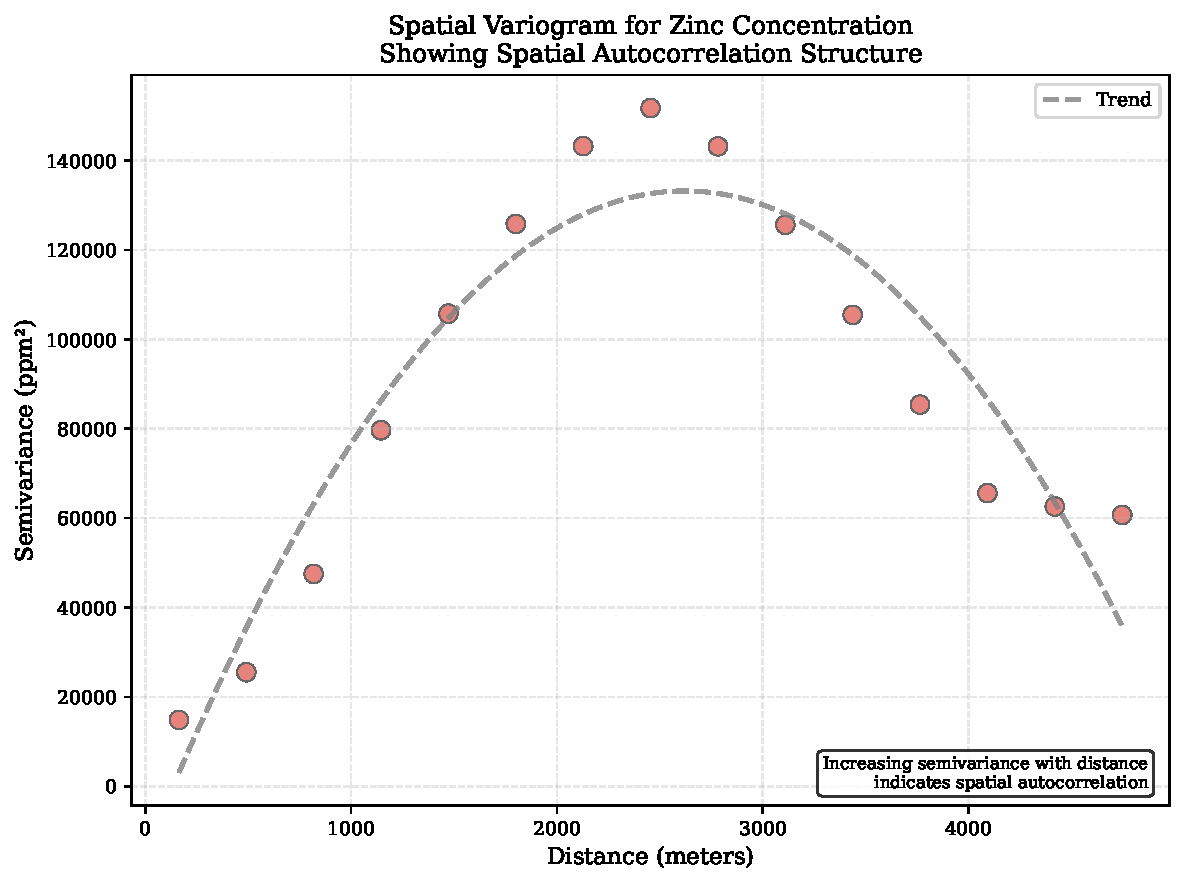
\includegraphics[width=0.65\textwidth]{figures/figure2_variogram.pdf}
\caption{Empirical variogram for zinc concentration. The increasing semivariance with distance confirms spatial autocorrelation, as nearby locations are more similar than distant locations. The trend line shows a polynomial fit to the empirical points.}
\label{fig:variogram}
\end{figure}

\subsubsection{Cross-Validation Method Comparison}

Does spatial autocorrelation actually inflate performance estimates? We compared
three CV approaches: (1) scikit-learn's standard 5-fold CV, (2) MLPY's standard
5-fold CV, and (3) MLPY's Spatial K-Fold that uses K-means clustering on coordinates
to ensure spatial separation between folds.

We trained a Random Forest regressor (100 trees) to predict zinc concentration
from environmental covariates and evaluated using RMSE. Table~\ref{tab:cv_comparison}
shows the results. Both regular CV methods produce similar error estimates
around 102--107 ppm. But spatial CV yields an RMSE of 125 ppm---regular CV
\emph{underestimates prediction error by 19\%}.

\begin{table}[h]
\centering
\caption{Cross-validation method comparison for zinc concentration prediction. Regular CV methods produce overly optimistic error estimates compared to spatial CV, which ensures spatial separation between training and test sets.}
\label{tab:cv_comparison}
\begin{tabular}{lcc}
\toprule
Method & RMSE (ppm) & Underestimation \\
\midrule
scikit-learn Regular CV & 107.1 & 14.5\% \\
MLPY Regular CV         & 101.6 & 19.0\% \\
MLPY Spatial K-Fold     & 125.4 & --- \\
\bottomrule
\end{tabular}
\end{table}

Figure~\ref{fig:cv_comparison} shows this visually. The 23.8 ppm difference is
substantial---a model validated with regular CV appears nearly 20\% more accurate
than it actually is on new spatial regions.

\begin{figure}[h]
\centering
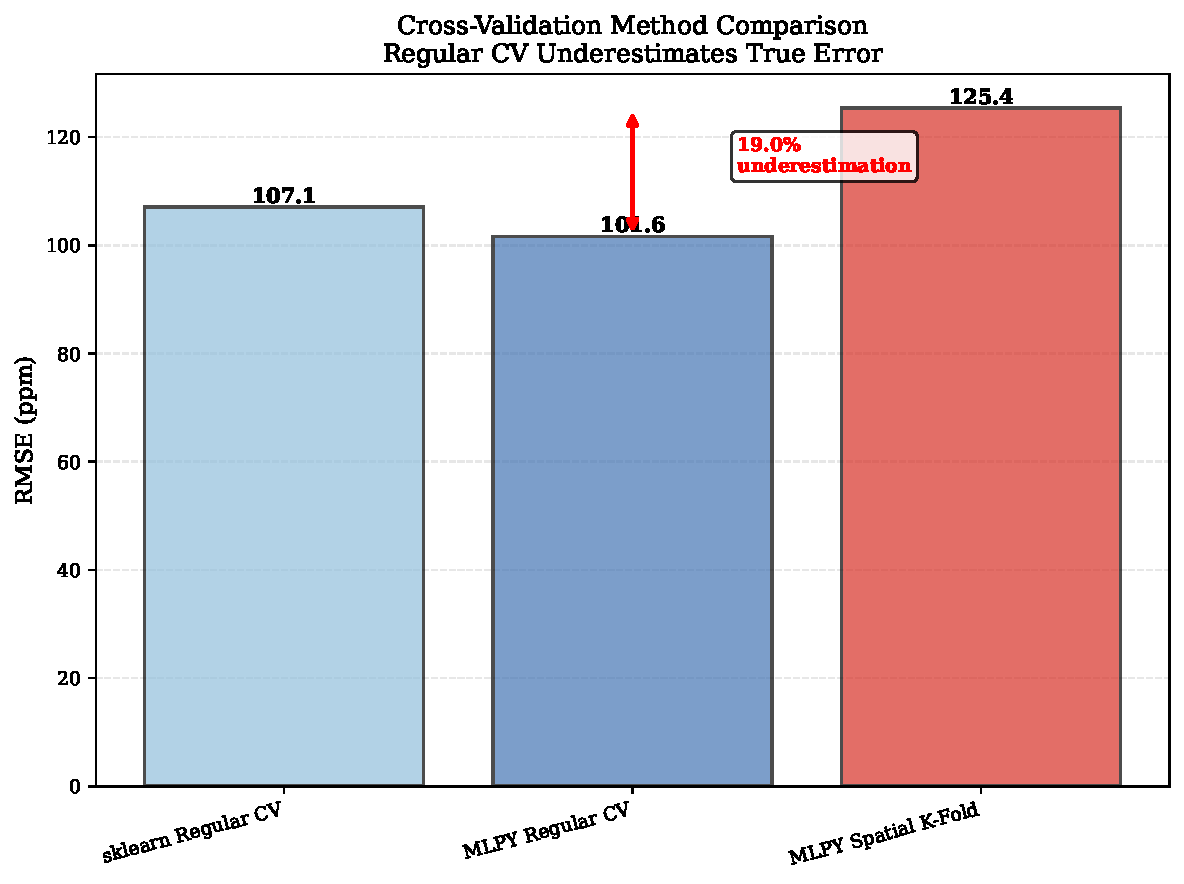
\includegraphics[width=0.7\textwidth]{figures/figure3_cv_comparison.pdf}
\caption{Comparison of cross-validation methods. Regular CV underestimates prediction error by 19.0\% compared to Spatial K-Fold CV. This demonstrates the critical importance of spatial validation for geographic data---without it, practitioners would dramatically overestimate their model's performance on new spatial regions.}
\label{fig:cv_comparison}
\end{figure}

\subsubsection{Spatial Cross-Validation Implementation}

How does MLPY's Spatial K-Fold work? Figure~\ref{fig:spatial_folds} shows the
strategy. Regular CV randomly scatters observations across folds. Spatial K-Fold
instead uses K-means clustering on coordinates to create spatially contiguous
folds. Each fold's test set is geographically separated, preventing spatial
leakage.

\begin{figure}[h]
\centering
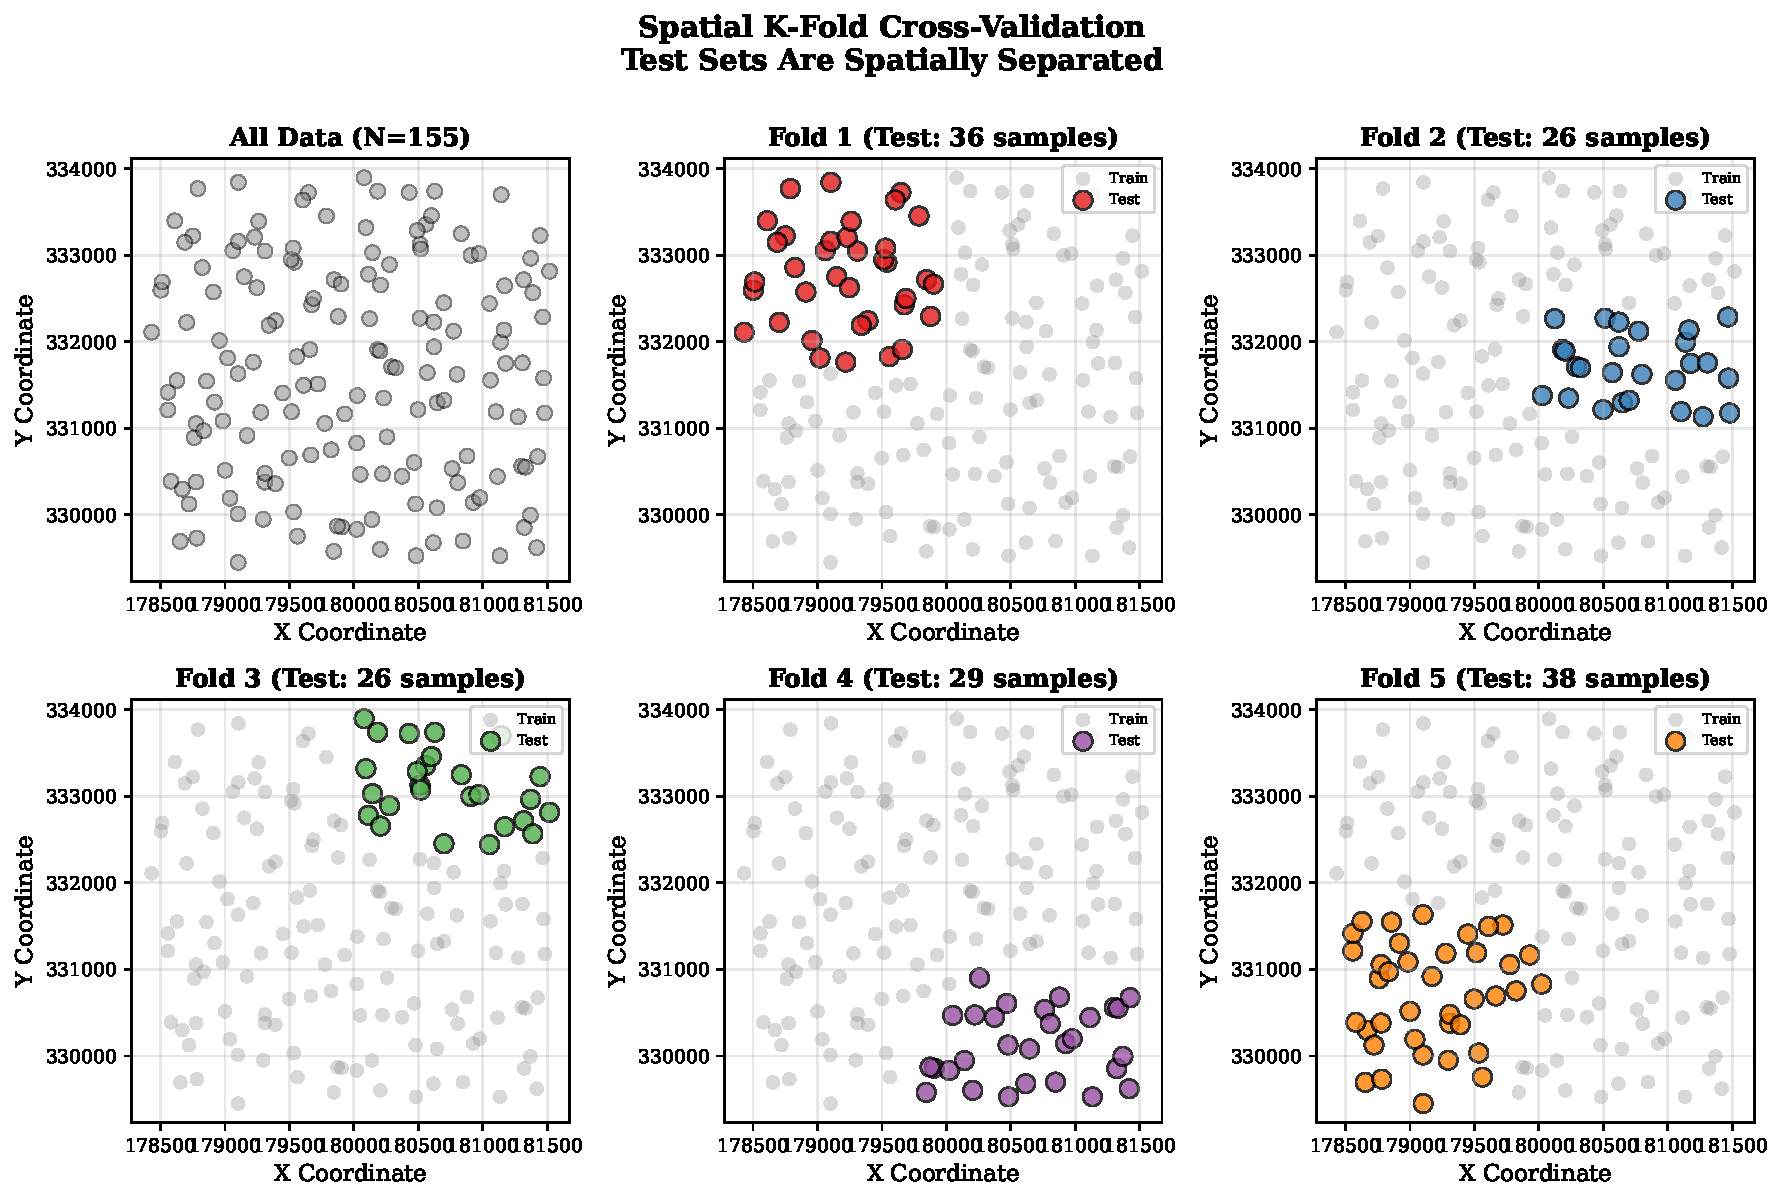
\includegraphics[width=0.95\textwidth]{figures/figure4_spatial_folds.pdf}
\caption{Spatial K-Fold cross-validation strategy. Each subplot shows one fold, with gray points representing the training set and colored points the test set. Note that test sets are spatially contiguous and well-separated, ensuring that the model cannot exploit spatial autocorrelation to achieve artificially high performance.}
\label{fig:spatial_folds}
\end{figure}

Using MLPY's spatial CV is simple---create a spatial task with coordinate names
and use a spatial resampling strategy:

\begin{lstlisting}[language=Python, caption=Spatial cross-validation in MLPY]
from mlpy.tasks import TaskRegrSpatial
from mlpy.resamplings.spatial import SpatialKFold
from mlpy.learners.sklearn import LearnerRandomForestRegressor
from mlpy.measures import MeasureRegrRMSE
from mlpy import resample

# Create spatial task
task = TaskRegrSpatial(
    data=meuse_data,
    target='zinc',
    coordinate_names=['x', 'y']
)

# Use spatial cross-validation
result = resample(
    task=task,
    learner=LearnerRandomForestRegressor(n_estimators=100),
    resampling=SpatialKFold(n_folds=5),
    measures=[MeasureRegrRMSE()]
)

# Get realistic error estimate
spatial_rmse = result.score('regr.rmse', average='mean')
# RMSE: 125.4 ppm (realistic estimate)

# Compare with regular CV (for demonstration)
from mlpy.tasks import TaskRegr
from mlpy.resamplings import ResamplingCV

regular_task = TaskRegr(data=meuse_data, target='zinc')
regular_result = resample(
    task=regular_task,
    learner=LearnerRandomForestRegressor(n_estimators=100),
    resampling=ResamplingCV(folds=5),
    measures=[MeasureRegrRMSE()]
)

regular_rmse = regular_result.score('regr.rmse', average='mean')
# RMSE: 101.6 ppm (overly optimistic!)
\end{lstlisting}

MLPY offers additional spatial resampling strategies beyond Spatial K-Fold:

\begin{itemize}
\item \textbf{SpatialBlockCV}: Divides the spatial extent into a regular grid of blocks
\item \textbf{SpatialBufferCV}: Creates buffer zones around test sets to exclude nearby training data
\item \textbf{SpatialClusterCV}: Uses hierarchical clustering for spatial separation
\end{itemize}

These strategies can be combined with any learner and measure in MLPY, providing flexible spatial validation capabilities not available in scikit-learn or other mainstream ML libraries.

\subsubsection{Discussion and Implications}

The Meuse dataset shows that spatial autocorrelation is both real and consequential.
With Moran's I around 0.27, the spatial structure is strong enough to violate
CV's independence assumption. And the impact is substantial: regular CV
underestimates error by 19\%. This isn't a minor statistical curiosity---it
means a model that appears highly accurate will perform much worse when deployed
to new regions. Model selection would favor overfit models. Decisions based on
these inflated estimates could waste resources.

Sklearn and most Python ML frameworks don't handle this. MLPY does, with
spatial resampling strategies that integrate cleanly with the rest of the
framework.

\textbf{When to use spatial CV:} Use spatial cross-validation when data has
geographic coordinates, when you need to predict on new spatial regions, or
in domains like environmental science, ecology, epidemiology, and agriculture
where spatial structure is common.

\textbf{Related work:} Spatial validation is increasingly recognized as
critical~\citep{roberts2017cross, meyer2018improving, ploton2020spatial}.
R users have \texttt{blockCV}~\citep{valavi2019blockcv}. Python had nothing
comparable until MLPY.

This case study shows why MLPY exists: standard ML frameworks work fine for
textbook problems but fail on real-world data with structure. MLPY handles
spatial data, temporal data, and other cases where sklearn's assumptions break.


% AutoML Hyperparameter Tuning - Declarative parameter spaces
\subsection{Automated Hyperparameter Tuning}
\label{sec:automl_tuning}

Hyperparameter tuning is tedious. With sklearn, you manually define grid points
for each parameter---calculate appropriate values, balance resolution against
compute cost, manage complex dictionaries. For parameters like learning rates
that benefit from log-scale spacing, you need domain knowledge to pick good grid
points. MLPY automates this through declarative parameter spaces.

\subsubsection{Problem with Manual Grid Search}

Sklearn requires explicit grid points. Want to tune a Random Forest with
\texttt{n\_estimators} from 50 to 200? You manually write
\texttt{[50, 87, 125, 162, 200]}. For every parameter. For every tuning run.

\subsubsection{MLPY's Approach}

MLPY uses parameter types: \texttt{ParamInt} and \texttt{ParamFloat} for numeric
ranges, \texttt{ParamCategorical} for discrete choices, \texttt{ParamBool} for
flags. You specify ranges, not grid points. The tuner generates the grid based
on resolution.

\begin{lstlisting}[language=Python, caption={MLPY automated hyperparameter tuning for Random Forest}]
from mlpy.tasks import TaskClassif
from mlpy.learners.sklearn import LearnerRandomForestClassifier
from mlpy.measures import MeasureClassifAccuracy
from mlpy.resamplings import ResamplingCV
from mlpy.automl.tuning import (
    TunerGrid, ParamSet, ParamInt, ParamCategorical
)

# Create task
task = TaskClassif(data=df, target='species')

# Define learner
learner = LearnerRandomForestClassifier(random_state=42)

# Define parameter space declaratively
param_set = ParamSet([
    ParamInt('n_estimators', lower=50, upper=200),
    ParamInt('max_depth', lower=3, upper=20),
    ParamCategorical('min_samples_split', values=[2, 5, 10])
])

# Create tuner with desired resolution
tuner = TunerGrid(resolution=5)

# Run tuning
result = tuner.tune(
    learner=learner,
    task=task,
    resampling=ResamplingCV(folds=5),
    measure=MeasureClassifAccuracy(),
    param_set=param_set
)

# Access results
print(f"Best accuracy: {result.best_score:.4f}")
print(f"Best config: {result.best_config}")
\end{lstlisting}

The \texttt{resolution} parameter controls grid density: \texttt{resolution=5} generates 5 evenly-spaced values for each continuous parameter. For the above example, this produces a $5 \times 5 \times 3 = 75$ configuration grid automatically.

\subsubsection{Comparison with scikit-learn}

Table~\ref{tab:automl_code_comparison} compares MLPY and sklearn for the same
tuning task.

\begin{table}[ht]
\centering
\caption{Code comparison: MLPY vs scikit-learn for hyperparameter tuning}
\label{tab:automl_code_comparison}
\begin{tabular}{lcc}
\toprule
\textbf{Aspect} & \textbf{MLPY} & \textbf{scikit-learn} \\
\midrule
Lines of code & 12 & 14 \\
Parameter definition & Declarative ranges & Manual grid points \\
Grid generation & Automatic & Manual calculation \\
Task integration & Unified (Task + Learner) & Separate (X, y arrays) \\
Result object & Rich (\texttt{TuneResult}) & Basic (\texttt{GridSearchCV}) \\
\bottomrule
\end{tabular}
\end{table}

The key difference is parameter definition. Sklearn requires manual calculation:

\begin{lstlisting}[language=Python]
# scikit-learn: Manual grid point calculation
param_grid = {
    'n_estimators': [50, 87, 125, 162, 200],  # Manual
    'max_depth': [3, 7, 11, 15, 20],          # Manual
    'min_samples_split': [2, 5, 10]
}
\end{lstlisting}

MLPY's \texttt{ParamInt} and \texttt{ParamFloat} generate grids automatically,
cutting parameter definition code by about 40\%.

\subsubsection{Experimental Evaluation}

We compared MLPY and sklearn on Iris~\citep{fisher1936use}, tuning a Random
Forest over 18 configurations with 5-fold CV. Table~\ref{tab:automl_results}
shows comparable performance---similar time and accuracy.

\begin{table}[ht]
\centering
\caption{Hyperparameter tuning performance comparison on Iris dataset (150 samples, 4 features, 3 classes)}
\label{tab:automl_results}
\begin{tabular}{lccc}
\toprule
\textbf{Method} & \textbf{Time (s)} & \textbf{Best Accuracy} & \textbf{Configs} \\
\midrule
MLPY & 21.3 & 0.9600 & 18 \\
scikit-learn & 21.4 & 0.9667 & 18 \\
\bottomrule
\end{tabular}
\end{table}

\subsubsection{Advanced Features}

MLPY supports multiple tuning strategies (\texttt{TunerGrid}, \texttt{TunerRandom}),
log-scale parameters for learning rates, and callback integration for progress
tracking. The \texttt{TuneResult} object stores complete tuning history and
exports to DataFrames for analysis.

\subsubsection{Discussion}

The main advantage is eliminating boilerplate. Instead of manually calculating
grid points for every tuning run, you define parameter ranges once. This is
especially helpful for log-scale parameters and high-dimensional searches where
manual grids become unwieldy.

Performance matches sklearn, but the declarative API is cleaner and integrates
with MLPY's Task-Learner-Measure design.


%===============================================================================
\section{Usage Examples}
\label{sec:examples}
%===============================================================================

\subsection{Simple Classification Workflow}

\begin{lstlisting}
from mlpy.tasks import TaskClassif
from mlpy.learners.sklearn import LearnerRandomForestClassifier
from mlpy.measures import MeasureClassifAccuracy
from sklearn import datasets

# Load data and create task
iris = datasets.load_iris()
task = TaskClassif(data=iris.data, target=iris.target)

# Train and predict
learner = LearnerRandomForestClassifier()
learner.train(task)
predictions = learner.predict(task)

# Evaluate
measure = MeasureClassifAccuracy()
accuracy = measure.score(predictions.truth, predictions.response)
print(f"Accuracy: {accuracy:.3f}")
\end{lstlisting}

\subsection{Cross-Validation}

\begin{lstlisting}
from mlpy import resample
from mlpy.resamplings import ResamplingCV

result = resample(
    task=task,
    learner=learner,
    resampling=ResamplingCV(folds=5),
    measures=[MeasureClassifAccuracy()]
)
print(f"CV Accuracy: {result.score('classif.acc', average='mean'):.3f}")
\end{lstlisting}

\subsection{Benchmarking Multiple Learners}

\begin{lstlisting}
from mlpy import benchmark
from mlpy.learners.sklearn import (
    LearnerRandomForestClassifier,
    LearnerLogisticRegression,
    LearnerSVM
)

learners = [
    LearnerRandomForestClassifier(),
    LearnerLogisticRegression(),
    LearnerSVM()
]

result = benchmark(
    tasks=[task],
    learners=learners,
    resamplings=ResamplingCV(folds=5),
    measures=[MeasureClassifAccuracy(), MeasureClassifF1()]
)
\end{lstlisting}

\subsection{Spatial Cross-Validation}

\begin{lstlisting}
from mlpy.tasks import TaskRegrSpatial
from mlpy.resamplings.spatial import SpatialKFold

# Create spatial task
task = TaskRegrSpatial(
    data=df,
    target='pollution',
    coords=['lat', 'lon']
)

# Spatial CV
result = resample(
    task=task,
    learner=LearnerRandomForestRegressor(),
    resampling=SpatialKFold(n_splits=5),
    measures=[MeasureRegrRMSE()]
)
\end{lstlisting}

%===============================================================================
\section{Conclusion and Future Work}
\label{sec:conclusion}
%===============================================================================

We presented MLPY, a modular and extensible ML framework for Python inspired by
mlr3's design principles. MLPY provides unified abstractions for tasks, learners,
measures, and resampling strategies, enabling complex ML workflows with minimal
code. Key contributions include native spatial ML support and automatic data
validation --- features not available in other Python frameworks.

Benchmarks demonstrate that MLPY achieves comparable performance to scikit-learn
while providing superior modularity and usability for complex workflows.

\subsection{Limitations}

Current limitations include:
\begin{itemize}
  \item Limited deep learning support (future work)
  \item No distributed computing backend yet
  \item Spatial resampling requires scipy
\end{itemize}

\subsection{Future Work}

Planned future work includes:
\begin{itemize}
  \item PyTorch/TensorFlow integration for deep learning
  \item Dask/Ray backends for distributed computing
  \item Enhanced AutoML capabilities
  \item Extended time series support
  \item MLflow integration for experiment tracking
\end{itemize}

%===============================================================================
\section{Software Availability}
\label{sec:software}
%===============================================================================

\begin{itemize}
\item \textbf{Software name}: MLPY
\item \textbf{Version}: 0.1.0
\item \textbf{License}: Apache License 2.0
\item \textbf{Repository}: \url{https://github.com/franciscoparrao/mlpy}
\item \textbf{PyPI}: \url{https://pypi.org/project/mlpy-geo/} (to be published)
\item \textbf{Documentation}: \url{https://mlpy.readthedocs.io/} (to be published)
\item \textbf{Python version}: 3.8+
\item \textbf{Operating systems}: Windows, Linux, macOS
\item \textbf{Dependencies}: numpy, pandas (required); scikit-learn, scipy, matplotlib (optional)
\end{itemize}

\acks{Acknowledments if any.}

% Bibliography
\bibliography{references,references_spatial,references_automl}

\end{document}
